\documentclass[border=8pt]{standalone}
\usepackage[utf8]{inputenc}\usepackage[T1]{fontenc}\usepackage{lmodern}\usepackage{tikz}\usetikzlibrary{arrows.meta,positioning}
\begin{document}
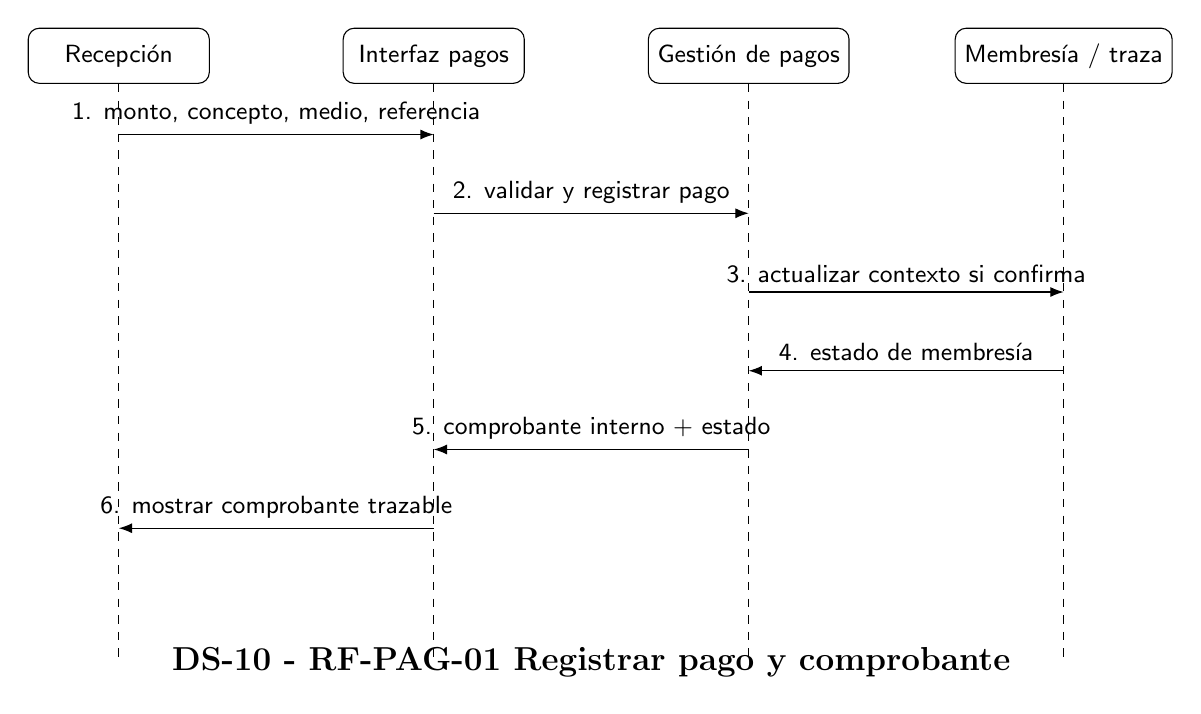
\begin{tikzpicture}[font=\sffamily\small,>=Latex]
\node[draw,rounded corners,minimum width=2.3cm,minimum height=.7cm] (rec) at (0,0) {Recepción};
\node[draw,rounded corners,minimum width=2.3cm,minimum height=.7cm] (ui) at (4,0) {Interfaz pagos};
\node[draw,rounded corners,minimum width=2.5cm,minimum height=.7cm] (svc) at (8,0) {Gestión de pagos};
\node[draw,rounded corners,minimum width=2.6cm,minimum height=.7cm] (mem) at (12,0) {Membresía / traza};
\foreach \n in {rec,ui,svc,mem}{\draw[dashed] (\n.south) -- ++(0,-7.3);}
\draw[->] (0,-1) -- node[above]{1. monto, concepto, medio, referencia} (4,-1);
\draw[->] (4,-2) -- node[above]{2. validar y registrar pago} (8,-2);
\draw[->] (8,-3) -- node[above]{3. actualizar contexto si confirma} (12,-3);
\draw[->] (12,-4) -- node[above]{4. estado de membresía} (8,-4);
\draw[->] (8,-5) -- node[above]{5. comprobante interno + estado} (4,-5);
\draw[->] (4,-6) -- node[above]{6. mostrar comprobante trazable} (0,-6);
\node[font=\bfseries\large] at (6,-7.7) {DS-10 - RF-PAG-01 Registrar pago y comprobante};
\end{tikzpicture}
\end{document}
